%%%%%%%%%%%%%%%%%%%%%%%%%%%%%%%%%%%%%%%%%%%%%%%%%%%%%%%%%%%%%%%%%%%%%%%%%%%%%%%%%%%%%
\section{Future Directions: Multi-Messenger Dark Matter Search}\label{sec:future}
%%%%%%%%%%%%%%%%%%%%%%%%%%%%%%%%%%%%%%%%%%%%%%%%%%%%%%%%%%%%%%%%%%%%%%%%%%%%%%%%%%%%%

\begin{figure}[h]
    \centering{
        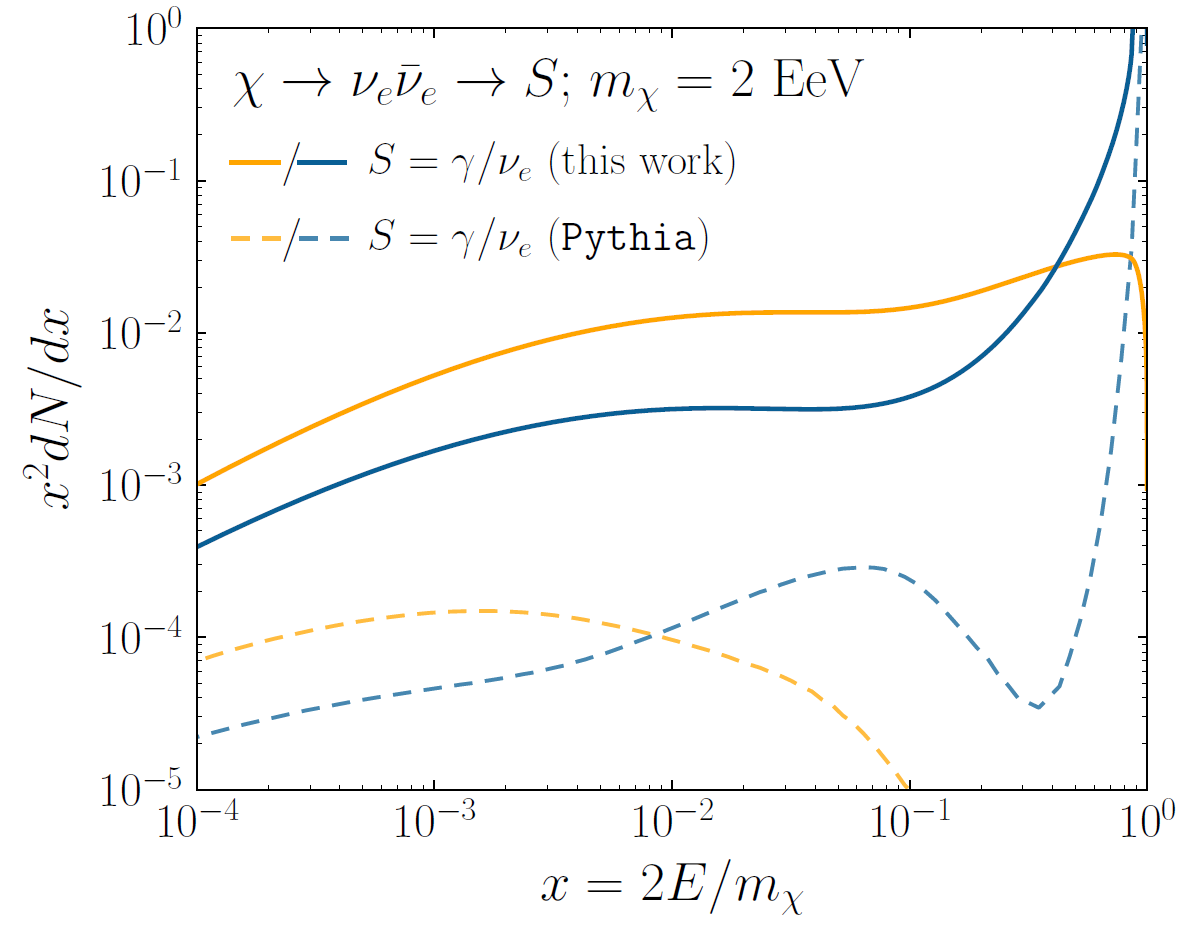
\includegraphics[scale=0.4]{figures/hdm_gamma_nu.png}
    }
    \caption{The $\nu_e$ and $\gamma$ spectrum at production from the decay of a 2 EeV DM particle to \parpar{\nu_e}. Solid lines are from the work of Nick Rodd et al. \cite{Rodd:HDM_spec}. Dashed lines are previous models produced by the particle physics framework \textbf{PYTHIA} \cite{PYTHIA}. Notice that the flux for both $\nu_e$ and $\gamma$ are significantly larger than previously predicted, especially at low energies. Similar changes are seen in DM masses above the electroweak scale.}
    \label{fig:nu_and_gam}
\end{figure}

As was shown previously in \Cref{sec:glory_duck} and \Cref{sec:multithread}, a fast and robust analysis was built in HAWC that can share tools with collaborators in particle astrophysics.
A formalism for combining common DM observations has been established.
These works, \Cref{sec:glory_duck}, and accelerations, \Cref{sec:multithread}, has laid the groundwork for faster DM searches without sacrificing on the scientific rigor.

\begin{figure}[t]
    \centering{
        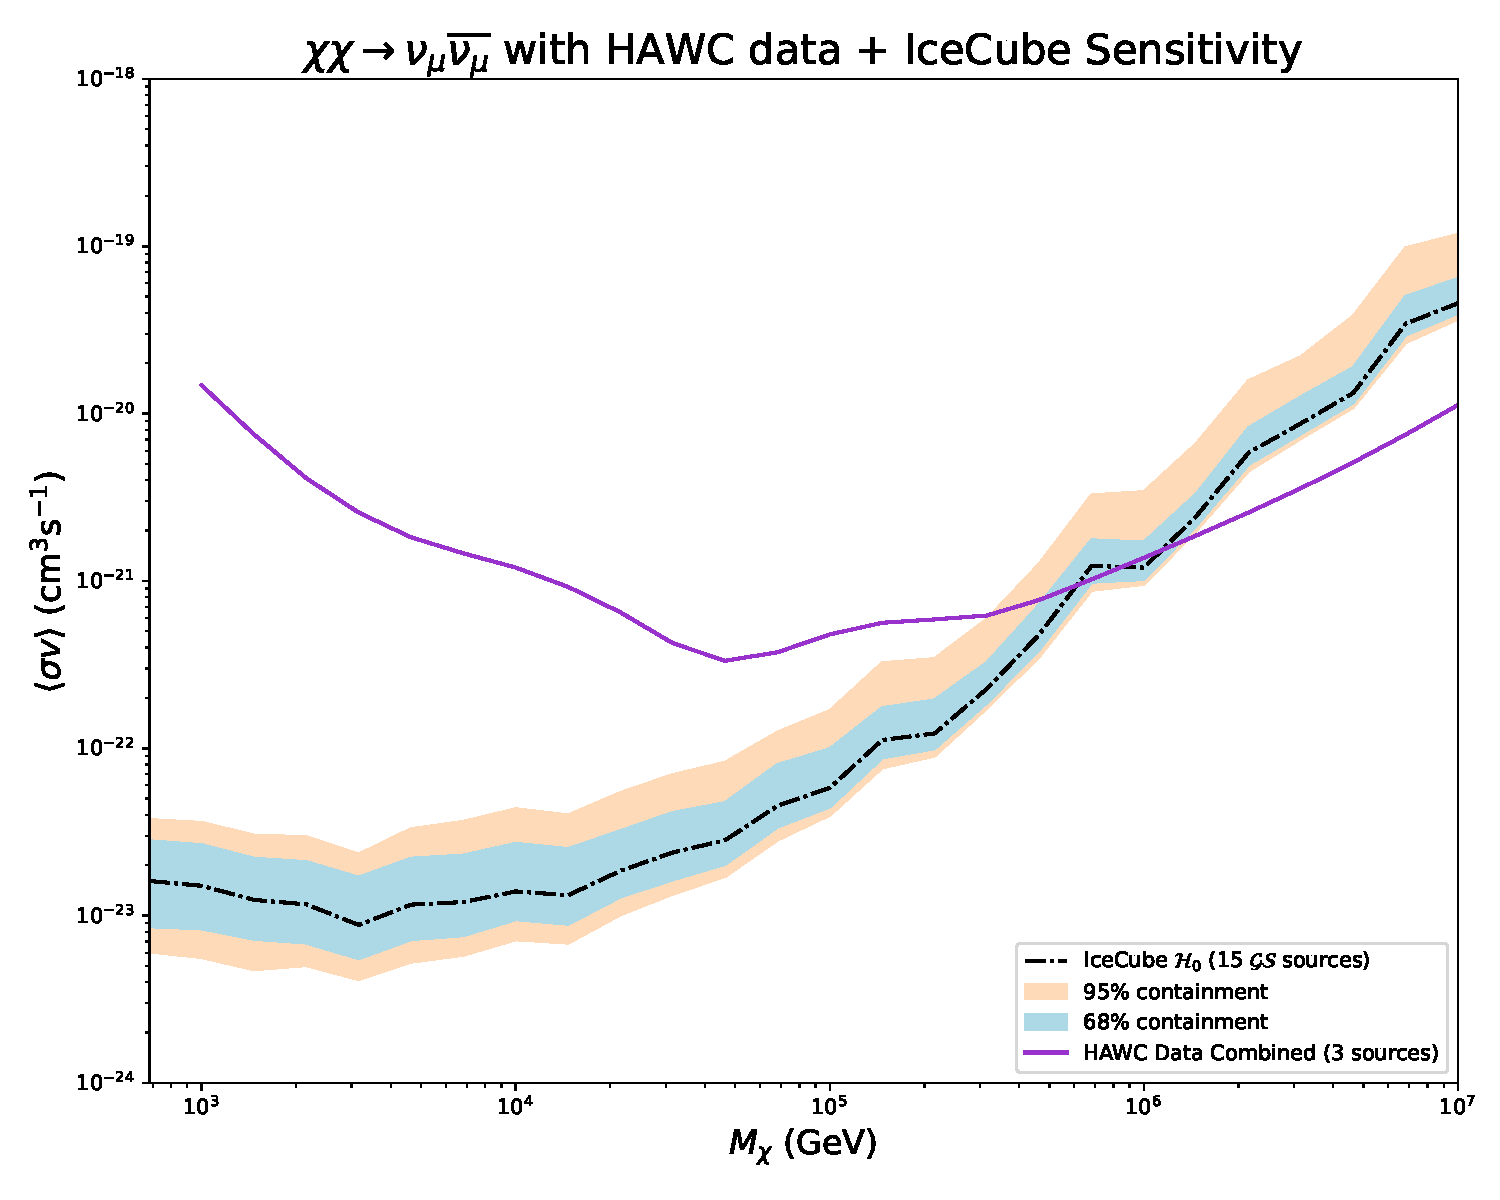
\includegraphics[scale=0.6]{figures/numunumu_hawcWic3_sens.pdf}
    }
    \caption{(purple line) HAWC 95\% confidence limit on \sv~ for WIMP DM for 1 TeV to 10 PeV DM mass. HAWC data is from observations of 3 sources: Coma Berenices, Segue 1, and Sextans. (Dashed black line) IceCube median 95\% confidence limit on \sv~over 300 background trials. Colored bands around IceCube sensitivity are the 68\% (light blue) and 95\% (peach) containment bands. The median IceCube value and HAWC data are most similar in the $m_\chi \approx 1$ PeV region.}
    \label{fig:nuDuck_sens}
\end{figure}

Within IceCube, the first DM annihilation search towards dSphs in over a decade is starting, \Cref{sec:ic3_dm}.
This work was developed with the long-term goal of combining it with the gamma-ray data for a multi-messenger DM search.
There is already promising developments in DM phenomenology in this regard.
\Cref{fig:nu_and_gam} is the headline figure from HDMSpectra \cite{Rodd:HDM_spec} for a DM decay ($\chi \rightarrow$\parpar{\nu_e}) spectrum in $\nu_e$~and $\gamma$.
What is intriguing from this publication is that although photons more readily interact with our detector than neutrinos, the expected photon spectrum is soft enough to be difficult to discern from the background.
Whereas, IceCube has exceptional sensitivity for hard neutrino spectra, see \cref{fig:icDM_stact_numu_TS,fig:icDM_sensitivity_2of2}.
Additionally, the Earth plays a role in reducing IceCube's neutrino sensitivity, see \cref{fig:icDM_dec_study} and \cite{IC3:Earth_Attenuation}.
These known behaviors suggested a potentially powerful partnership between HAWC and IceCube.

Preliminary work was done to combine HAWC and IceCube data for a multi-messenger DM search.
Through background simulation, \Cref{sec:ic3_dm} showed that IceCube variables behave mostly like normal variables distributed as a $\chi^2$ distribution with 1 degree of freedom.
For IceCube the statistical framework for setting confidence limits first made by Fermi-LAT \cite{FermiLAT:dm1}, and later Glory Duck, \cref{sec:gd_joint_llh}.
For this combination analysis, IceCube adopts the 95\% confidence limit standard defined in \cref{eq:hawc_cl95} with a likelihood combination using \cref{eq:gdJointLLH}.
This differs from the 90\% confidence limit considered standard within IceCube and used for \Cref{sec:ic3_dm}.
This statistical definition is standard for HAWC and requires no additional changes than what was presented in \Cref{sec:multithread}.

Sensitivities are calculated for IceCube on 300 background trials. \Cref{fig:nuDuck_sens} presents the median, 68 and 95 percentile containment on the confidence limit with IceCube NST; dataset described in \cref{sec:icDM_data_bkgd}.
The source and model selection for IceCube is identical to \cref{sec:ic3_study_selection}.
Confidence limits on HAWC data are calculated using the methods and dataset from \cref{sec:mtd_srcs_y_chan} and DM density model (\GS) methods from \cref{sec:gd_srcs_y_chan}.
HAWC does not have an unblinding process, like IceCube.
Permission to unblind has not been granted, so only sensitivities are included for now.
It is unclear when unblinding will be granted for this combination as this depends heavily on the publication of the work in \Cref{sec:multithread,sec:ic3_dm}.
Yet, they all share much of the same machinery, so it is not expected to be long after the works are published.

\Cref{fig:nuDuck_sens} features IceCube's sensitivity superimposed on HAWC's 95\% confidence limit on DM annihilation: $\chi\chi \rightarrow$ \parpar{\nu_\mu} at a 100\% BR.
We can see that IceCube's sensitivity is complimented well by HAWC's confidence limit in the DM mass region above and around 1 PeV.
More complex models with diverse BRs are possible and the method of analysis would require a substitution as was described in \cref{sec:break_it}.

A mock combination between HAWC and IceCube has been performed.
This mock run was made for the purpose of building the neutrino + gamma data pipeline for DM searches.
\Cref{fig:nuDuck_mockdata} shows a combined limit between HAWC data and an IceCube simulated background trial treated as data.
From this mock combination, it is evident that there is a powerful combination in the 1 PeV DM mass region.
There is an improvement to the combined limit to DM masses as far down to 100 TeV.
Furthermore, the improvement to this limit stay across two decades in DM mass.
This preliminary work is evidence of the strength in multi-messenger DM searches and motivates such a study between these instruments.

\begin{figure}
    \centering{
        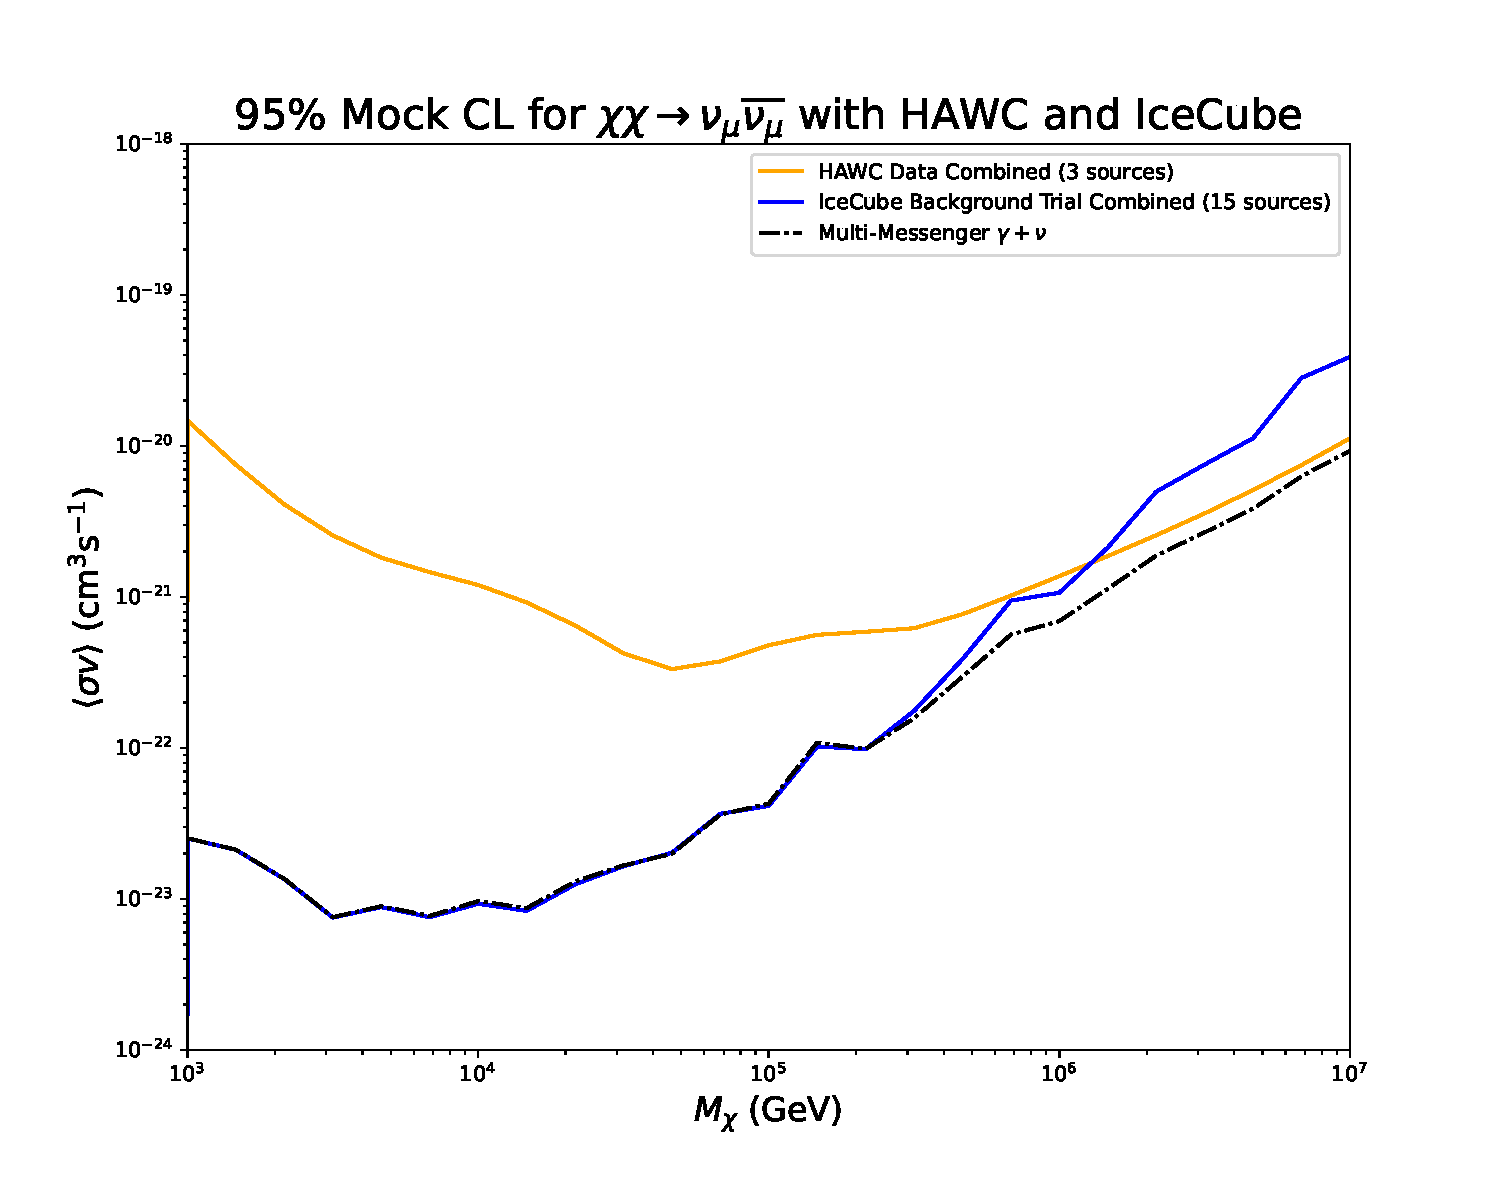
\includegraphics[scale=0.6]{figures/numunumu_mock_data.pdf}
    }
    \caption{(orange solid line) HAWC 95\% confidence limit on \sv~using data from 3 sources: Coma Berenices, Segue 1, and Sextans. (blue solid line) IceCube 95\% confidence limit on \sv~from one simulated background trial. (dashed black line) Combined 95\% confidence limit on \sv~with HAWC data and IceCube background trial. Combined limit is stronger than either IceCube and HAWC in the region $m_\chi > 200$ TeV. }
    \label{fig:nuDuck_mockdata}
\end{figure}

%%%%%%%%%%%%%%%%%%%%%%%%%%%%%%%%%%%%%%%%%%%%%%%%%%%%%%%%%%%%%%%%%%%%%%%%%%%%%%%%%%%%%
\section{Conclusions}\label{sec:conclusions}
%%%%%%%%%%%%%%%%%%%%%%%%%%%%%%%%%%%%%%%%%%%%%%%%%%%%%%%%%%%%%%%%%%%%%%%%%%%%%%%%%%%%%

This dissertation, "Leveraging Multi-Messenger Astrophysics for Dark Matter Searches", advances our quest to understand dark matter.
We used gamma-ray and neutrino observatories alongside advanced computational techniques.
Our goal was to enhance the search for dark matter within the universe.
We have made substantial strides in the search for dark matter using multi-messenger astrophysics.
The collaborative efforts of the Glory Duck team and the methodologies established in HAWC analyses have set a new precedent for the rapid and robust detection of dark matter signals.
My work within IceCube has revitalized the search for dark matter annihilation from dwarf spheroidal galaxies, laying the foundation for a comprehensive multi-messenger approach.

The Glory Duck project was a key part of this work.
It involved a multi-instrument analysis using gamma-ray telescopes. These included Fermi-LAT, H.E.S.S., MAGIC, VERITAS, and HAWC.
We focused on 20 dwarf spheroidal galaxies (dSphs).
The aim was to detect dark matter annihilation signals.
Although we found no significant deviations from the null hypothesis, we greatly improved search sensitivity.
We set stringent upper limits on the annihilation cross-section for dark matter candidates.
This effort represents a major advance, offering the most comprehensive constraints for WIMP dark matter search to date.
The potential synergy between IceCube and gamma-ray observatories like HAWC is particularly promising.
Preliminary work has demonstrated that by combining data from these observatories, we can significantly enhance our search sensitivity, especially in the dark matter mass region above 1 PeV.
This is clearly illustrated in Figure 7.2, where IceCube's sensitivity complements HAWC's confidence limit, and Figure 7.3, which showcases the improved limit that multi-messenger data offers.

Our exploration of multithreading techniques in HAWC analyses showed the benefits of computational methods.
By accelerating analysis time, we enhanced the efficiency of dark matter searches. This approach has set the stage for more ambitious studies.
It highlights the importance of computational innovation in addressing astrophysical challenges.

Furthermore, our work with IceCube's North Sky Track Data has broken new ground.
It aimed at detecting heavy dark matter annihilation.
We used parallel programming and spline fitting to improve and refine IceCube's  sensitivity.
This analysis is a step towards probing dark matter annihilation up to the PeV scale.
It demonstrates a significant sensitivity improvement compared to previous efforts.
The groundwork laid here is a strong foundation for future discoveries.

This dissertation highlights the potential of multi-messenger astrophysics and computational innovation in dark matter searches.
Each analysis has contributed to our understanding and capabilities.
Together, they showcase a progressive approach to astrophysical research by integrating observations from several gamma-ray and neutrino observatories.
Additionally, modern computational techniques such as multithreading were developed and deployed to greatly accelerate analyses in HAWC.
By harnessing the collective power of these observatories, we have created a legacy that will guide future collaborations.
Looking back, it's clear that our journey through the dark universe is far from complete.
The advances made herein beckon the next phase of discovery, where multi-messenger observations and analyses will illuminate further secrets of the dark universe.